\documentclass[
% opciók nélkül: egyoldalas nyomtatás, elektronikus verzió
% twoside,     % kétoldalas nyomtatás
% tocnopagenum,% oldalszámozás a tartalomjegyzék után kezdődik
]{thesis-ekf}
\usepackage[T1]{fontenc}
\PassOptionsToPackage{defaults=hu-min}{magyar.ldf}
\usepackage[magyar]{babel}
\usepackage{mathtools,amssymb,amsthm,pdfpages}
\usepackage{enumitem, graphicx, listings, xcolor, url}
\lstset{
	language=Python,
%	literate={ö}{{\"o}}1{ü}{{\"u}}1{ó}{{\'o}}1{ő}{{\H o}}1{ú}{{\'u}}1{ű}{{\H u}}1{é}{{\'e}}1{á}{{\'a}}1{í}{{\'i}}1{Ö}{{\"O}}1{Ü}{{\"U}}1{Ó}{{\'O}}1{Ő}{{\H O}}1{Ú}{{\'U}}1{Ű}{{\H U}}1{É}{{\'E}}1{Á}{{\'A}}1{Í}{{\'I}}1
	xleftmargin=1cm,
	xrightmargin=1cm,
	breaklines,
	tabsize=4,
	showstringspaces=false,
	frame=tlbr,
	postbreak=\hbox{$ \color{red}\hookrightarrow\ $},
	backgroundcolor=\color{gray!30},
	rulecolor=\color{green!50!black},
	keywordstyle=\bfseries\color{blue},
	commentstyle=\color{green!60!black}
	%morekeywords={None}
}
\footnotestyle{rule=fourth}

\newtheorem{tetel}{Tétel}[chapter]
\theoremstyle{definition}
\newtheorem{definicio}[tetel]{Definíció}
\theoremstyle{remark}
\newtheorem{megjegyzes}[tetel]{Megjegyzés}

\begin{document}
	\institute{Matematikai és Informatikai Intézet}
	\title{A kommunikációs gráfok modelljeinek vizsgálata Python programozási nyelvvel}
	\author{Mohai Ferenc\\programtervező informatikus BSc}
	\supervisor{Dr.~Kusper Gábor\\egyetemi docens}
	\city{Eger}
	\date{2022}
	
	\maketitle
	\tableofcontents
	
\chapter*{Bevezetés}
	\addcontentsline{toc}{chapter}{Bevezetés}
	A szakdolgozati szemináriumon, amikor hallottam Kusper Gábor tanár úr magyarázatát a kutatásról, annak eredményeiről, céljáról, felhasználásáról. és már akkor nagyon megtetszett a téma. A \textsc{SAT} megoldó széles körű felhasználásáról beszélgettünk. Korábbi előadásokon, gyakorlatokon is voltak tanáraim, akik ezt a témát felvetették, és már akkoriban meghozták a kedvemet hozzá. Amikor választanom kellett, nem volt nagy kérdés, hogy ez egy számomra érdekes téma, amivel szívesen dolgozok, és lehetőséget ad a fejlődésre.

	Szaktársammal, Rajna Franciskával csak mi ketten érdeklődtünk ebben a témában, úgyhogy mindenki örömmel beszélte meg a részleteket és közös megegyezéssel találtuk ki melyik ágát dolgozza ki a témának. Pozitív és energikus első benyomás után örömmel kezdtünk a munkának. Bíró Csaba és Balla Tamás tanár urakkal dolgoztunk a témával kapcsolatos házi TDK-hoz hasonló előadásokon és kutatásokon \cite{am} vettünk részt. Az egyik alkalommal egy plakátot is készítettünk, ezekkel megalapozva egy lendületes kezdést.
	
	Megbeszéltük hol szorul fejlesztésre a \textsc{SAT} megoldó, amin tudok programozással javítani. Valamint a korábbi általuk írt angol nyelvű szakirodalmakkal elsajátíthatom az elméleti hátteret, felzárkózhatok a jelenlegi helyzethez és ezeken dolgozva könnyedén belerázódjak a szakdolgozatom megfogalmazásába. Így kezdtem el a munkámat.
	
\chapter{Az alapok}
	
	A munkámat azzal kezdtem, hogy szakirodalmakat olvastam, fordítottam és értelmeztem, amiket korábban témavezetőim írtak, ez \az{\pageref{ssec-szakirodalom}}.~és a \az{\pageref{sec-szakirodalom-forditas}}.~oldalon olvasható. Anyagot gyűjtöttem és dolgoztam fel a \textsc{SAT} megoldókról. Ezekben megjelentek különböző definíciók, mint \ref{def-tautologia}.~definíció a tautológia, \az{\ref{def-cnf}}.~definíció a \textsc{CNF}, és \az{\ref{def-dnf}}.~definíció a \textsc{DNF}, valamint programozási nyelv, mint a Python \az{\ref{kif-python-programnyelv}}.~szakaszban és a WolframAlpha válasz motor \az{\ref{kif-wolframalpha-hasznalata}}.~szakaszban.
		
	\section{Szakirodalom}

	Alapfogalmak, definíciók:
	
	\begin{definicio}
		Atomi formula, röviden atom:  Azt mondjuk, hogy egy szimbólum atomi formula, vagy atom, akkor és csak akkor, ha egy kifejezést jelöl. Ilyen atomok, az igaz és hamis ítéletváltozók. Szimbólumuk általában az \emph{I} és \emph{H} betűk magyarul, de szoktuk használni az angol megfelelőjét is a \emph{T} és \emph{F} betűket.
	\end{definicio}

	\begin{definicio}
		Literál: Azt mondjuk, hogy egy szimbólum literál, akkor és csak akkor, ha egy atom, vagy annak negáltja.
	\end{definicio}

	\begin{definicio}		
		Jól formázott formula, röviden formula: Azt mondjuk, hogy egy szimbólum sorozat jól formázott formula, vagy formula, akkor és csak akkor, ha F formula a következő alakok egyikében van:
		\begin{enumerate}[label=\textit{(\alph*)}]
			\item A, ahol A egy atom;
			\item $ \neg A $, ahol A egy formula;
			\item $ (A \wedge B) $, ahol A és B formulák;
			\item $ (A \vee B) $, ahol A és B formulák;
			\item $ (A \implies B) $, ahol A és B formulák;
			\item $ (A \Leftrightarrow B) $, ahol A és B formulák.
		\end{enumerate}
		Minden formula a fenti esetek véges sokszori alkalmazásával áll elő.
	\end{definicio}

	\begin{definicio}
		Formula: Adott ítéletváltozónak egy véges, nem üres V halmaza.
		\begin{enumerate}
			\item Ítéletváltozó: ha $ A\in V $, akkor A formula.
			\item Negáció: ha A formula, akkor $\neg A $ is formula.
		\end{enumerate}
	\end{definicio}

	\begin{definicio}
		Operátor: Azt mondjuk, hogy egy szimbólum operátor, akkor és csak akkor, ha egy Formulán, klózon, vagy literálon módosítást végez, oly módon, hogy kiinduló állapotát megváltoztatja, megfelelő elő feltételek mellett. Azaz két ítéletváltozó értékéből, azokat értelmezve egy harmadik értéket eredményez.
	\end{definicio}
	
	\begin{definicio}
		Klóz, angolul clause: Azt mondjuk, hogy egy formula klóz, akkor és csak akkor, ha adott literáloknak és operátoroknak egy véges, nem üres, egynél több elemű W halmaza.

		Klózban értelmezve,
		\begin{enumerate}
			\item pozitív literál: ha $ B\in W $, és B egy pozitív literál.
			\item negatív literál: ha B pozitív literál, akkor $\neg B $ negatív literál.
			\item és operátor: ha $ B \wedge \neg B $, akkor $\wedge$ egy és operátor.
			\item vagy operátor: ha $ B \vee \neg B $, akkor $\vee$ egy vagy operátor.
		\end{enumerate}
		Pozitív vagy negatív literál is feltűnhet egy klózban, de sohasem egyszerre. Az is lehetséges, hogy valamelyik változó egyik formában sem tűnik fel egy klózban, hiszen egyszerűsíthetünk: $ B \wedge\neg B \equiv\emptyset $.
	\end{definicio}
	
	\begin{megjegyzes}
		Létezik konjunktív és diszjunktív klóz is. Vegyes egy klóz tartalma, ha vagy, valamint és operátorokat is tartalmaz.
	
		Diszjunktív klóz: Azt mondjuk, hogy $ l_{i} $ szimbólumok egy klózt alkotnak, akkor és csak akkor, ha minden $ l_{i} $ literál: $ l_{1}\vee\dots\vee l_{n} $
		
		Konjunktív klóz: Azt mondjuk, hogy $ l_{i} $ szimbólumok egy klózt alkotnak, akkor és csak akkor, ha minden $ l_{i} $ literál: $ l_{1}\wedge\dots\wedge l_{n} $
	\end{megjegyzes}

	\begin{definicio}
		Implikáció: Azt mondjuk hogy egy operátor implikáció, akkor és csak akkor, ha mindkét oldalán van egy literál, és egy harmadik literált állít elő a kettő értékéből, oly módon, hogy az összes bal oldali értékből pozitív literált állít elő, kivéve, ha a bal oldalán pozitív, a jobb oldalán negatív literál van.
		Mivel a negatív értékből nem következik a pozitív érték. Jelölése: $ A \implies B $
	\end{definicio}

	\begin{definicio}
		Ekvivalencia: Azt mondjuk, hogy egy operátor ekvivalencia, akkor és csak akkor, ha mindkét oldalán van egy literál, és egy harmadik literált állít elő a kettő értékéből, oly módon, hogy ha mindkét oldalán ugyan az a pólusú literál van, akkor pozitív literált állít elő, kivéve, ha eltérnek a pólusok. Jele: $ \equiv $
	\end{definicio}

	\begin{megjegyzes}
		Pólus alatt a negatív vagy pozitív jelzőt értjük.
	\end{megjegyzes}

	\begin{definicio}
		És operátor, más néven konjunkció: Azt mondjuk, hogy egy operátor konjunkció, akkor és csak akkor, ha mindkét oldalán van egy literál, és egy harmadik literált állít elő a kettő értékéből, oly módon, hogy ha mindkét oldalán pozitív literál van, akkor és csak akkor pozitív literált állít elő, különben negatív literált. Jele: $\wedge$
	\end{definicio}

	\begin{definicio}
		Vagy operátor, más néven diszjunkció: Azt mondjuk, hogy egy operátor diszjunkció, akkor és csak akkor, ha mindkét oldalán van egy literál, és egy harmadik literált állít elő a kettő értékéből, oly módon, hogy ha mindkét oldalán negatív literál van, akkor negatív literált állít elő, különben pozitív literált. Jele: $\vee$
	\end{definicio}

	\begin{definicio}\label{def-cnf} % megjegyzésbe kiemelni az angol megfelelőket? CNF DNF
		Konjunktív normál forma, röviden \textsc{knf}, angolul conjunctive normal form, röviden \textsc{CNF}: Azt mondjuk, hogy logikai formula konjunktív normál forma, akkor és csak akkor, ha egy vagy több klózt egymáshoz kötünk konjunkcióval.
	\end{definicio} % todo példákat cnfre, DNF-re

	\begin{definicio}\label{def-dnf}
		Diszjunktív normál forma, angolul disjunctive normal form, röviden \textsc{DNF}: Azt mondjuk, hogy logikai formula diszjunktív normál forma, akkor és csak akkor, ha egy vagy több klózt egymáshoz kötünk diszjunkcióval.
	\end{definicio}

	\begin{definicio}
		Interpretáció: Adott ítéletváltozóknak egy véges sok, nem üres V halmaza.
		Azt mondjuk, hogy a J hozzárendelés az F formula egy interpretációja, akkor és csak akkor, ha F minden atomjához vagy az igaz, vagy a hamis értéket rendeljük, de csak az egyiket.
	\end{definicio}

	\begin{definicio}\label{def-tautologia}
		Logikai törvény, más néven tautológia: Azt mondjuk, hogy az F formula logikai törvény, vagy tautológia, akkor és csak akkor, ha F minden interpretációjában igaz.
	\end{definicio}

	\begin{definicio}
		Logikai ellent mondás, angolul contradiction, unsatisfiable, röviden UNSAT: Azt mondjuk, hogy az F formula logikai ellentmondás, akkor és csak akkor, ha F minden interpretációjában hamis.
	\end{definicio}

	\begin{definicio}
		Kielégíthető, angolul satisfiable, röviden \textsc{SAT}: Azt mondjuk, hogy az F formula kielégíthető, akkor és csak akkor, ha F legalább egy interpretációjában igaz.
	\end{definicio}

	\begin{definicio}
		Hamissá tehető, angolul falseable: Azt mondjuk, hogy az F formula hamissá tehető, akkor és csak akkor, ha F legalább egy interpretációjában hamis. 
	\end{definicio}

	\begin{megjegyzes}
		Kielégítő ellentéte a logikai ellentmondás, mivel ha valami nem kielégíthető, akkor abból következik, hogy logikai ellentmondás.
		Hamissá tehető ellentéte a logikai törvény, mivel ha valami nem hamissá tehető, akkor abból következik, hogy logikai törvény.
	\end{megjegyzes}

	Igazság tábla: Oszloponként tartalmazza az összes atomot, ami a formulánkban van, és az utolsó oszlopban magát a formulát is. Soronként minden atomhoz értéket rendel, minden lehetséges sorrendben, és a formulába behelyettesítve kiszámítja a formula értékét. Az eredményét az utolsó oszlopból olvashatjuk ki.
	
	Logikai törvény, tautológia: Ezek segítségével felírhatunk olyan formulákat, és igazság táblákat, amelyek minden lehetséges esetre igaz értéket adnak eredményül. Az eredményekből könnyebben átláthatjuk, ha tautológiát kapunk.
	
	\begin{proof}\label{biz-tautologia}
		Tautológia: 
			
		Legyen $ a $ egy ítélet változó, akkor a következő formula eredménye mindig igaz lesz: $ a\vee\neg a $
		
		\begin{tabular}{|c|c|}
			\hline
			$ a $ & $ a=\neg a $ \\
			\hline
			I & I \\
			\hline
			H & I \\
			\hline
		\end{tabular}
	
		Legyen $ x $ és $ y $ egy-egy ítéletváltozó, akkor a következő formula eredménye mindig igaz lesz: $ x=y\vee x\ne y $
		
		\begin{tabular}{|c|c|c|}
			\hline
			$ x $ & $ y $ & $ x=y\vee x\ne y $ \\
			\hline
			I & H & I \\
			\hline
			H & I & I \\
			\hline
		\end{tabular}
	\end{proof}
	
	\textsc{SAT} probléma: A logikai kielégíthetőség egy olyan probléma, ami azt határozza meg, hogy létezik olyan interpretációja egy logikai formulának, ami kielégíti az adott logikai formulát.
	
	\textsc{SAT} megoldó, angolul \textsc{SAT} solver: Hosszú, és bonyolult \textsc{SAT} problémák megoldására képes.

	\subsection{A tanáraim ajánlása}\label{ssec-szakirodalom}
	\begin{definicio}
		Egy irányított gráf teljes, akkor és csak akkor, ha minden pár külön álló csúcsokból össze van kötve egy pár egyedi éllel (eggyel minden irányba). Egy irányított gráf erősen összetett, vagy erősen irányított gráf, akkor és csak akkor, ha van út minden csúcsból minden más csúcsba. Vegyük figyelembe, hogy a teljes gráf egyben erős is. És azt is, hogy az erősen irányított gráf tartalmaz egy kört, ami tartalmaz minden csúcsot \cite{am}.
	\end{definicio}

	\begin{definicio}
		Erősen összetett gráf, más néven erős gráf: Azt mondjuk, hogy egy gráf erős gráf, akkor és csak akkor, ha van út minden pár csúcs között.
	\end{definicio}
	
	\begin{definicio}
		Erősen összetett komponens, más néven erős komponens, angolul strongly connected component, röveiden \textsc{SCC}: Azt mondjuk, hogy egy részgráf erősen összetett komponens, akkor és csak akkor, ha egy irányított gráf maximális erősen összekötött részgráfja. 
	\end{definicio}
	
	\begin{definicio}
		Fekete hozzárendelés, más néven fekete klóz: Azt mondjuk, hogy egy klóz fekete klóz, akkor és csak akkor, ha a gráf minden csúcsának negáltja megtalálható benne.
	\end{definicio}
	
	\begin{definicio}
		Fehér hozzárendelés, más néven fehér klóz: Azt mondjuk, hogy egy klóz fehér klóz, akkor és csak akkor, ha a gráf minden csúcsa megtalálható benne.
	\end{definicio}

 	\section{Draw.io képszerkesztő}

	A \cite{link-drawio} weboldalon elérhető \textsc{XML} alapú képszerkesztő. Egy olyan webes grafikus felületet ad, ami gráfok, diagramok, uml, use-case ábrák, képek, és még sok más forma megszerkesztését teszi lehetővé. Ha akarjuk le is tölthetjük ingyenesen az asztali alkalmazást, ami szélesebb körben, gyorsabban és precízebben működik, mint a webes felület. Gyorsabb a fájlok kezelése, szerkesztése is.
	
	Rengeteg alapértelmezett alakzatot találunk benne, használata egyszerű, és könnyen ráérez az ember. Körülbelül 3 éve hallottam erről az alkalmazásról, talán Troll Ede tanár úr mutatta be nekünk még Bevezetés az informatikába című órán. Azóta rengeteg umlt, use-case-tt és egyéb hasznos dolgot szerkesztettem már meg, csak úgy, mint az összes gráfot a jelenlegi dokumentumban.
	
	\section{WolframAlpha válasz motor}
	A Wolfram nyelv általános, több paradigmás programozási nyelv az alapja. Ami a hangsúlyt a szimbolikus számításra, a funkcionális programozásra, a szabályalapú programozásra helyezi, valamint képes tetszőleges struktúrákat és adatokat alkalmazni. Ezekre az alapokra épül a WolframAlpha tudás számító és válasz motor. Képes közvetlenül válaszolni a tényszerű kérdésekre azáltal, hogy külső forrásból származó adatokból számítja ki a választ.
	
	Mi arra tudjuk használni, a saját weboldalán keresztül \cite{link-wolframalpha}, hogy beviteli mezőbe logikai formulát adunk át neki. Válasznak vissza adja megformázva, amit beírtunk, annak igazság tábláját, normál formáit, logikai áramkörét, Venn diagrammát és az igazság sűrűségét.
	
	Így könnyen leellenőrizhető, hogy a logikai formula amit beírtunk az tautológia-e. Ezt az igazságtábla utolsó oszlopából láthatjuk.
	
		\subsection{Használata}\label{kif-wolframalpha-hasznalata}
	Akár szavak keresésére is alkalmas, nagyon széles körű, intelligens kereső motor. Képes megkeresni, akár szavak rímjétől egészen az egyszerű és a bonyolult matematikai képleteken át át, a nagyon összetett logikai formulákig bármire válaszolni. Ehhez csak tudnunk kell a formátumot, amiben dolgozunk. Egy szó begépelésével, annak jelentését adja vissza, hozzá tartozó szinonimákat, nyelvtani felépítését, használatát az évek során, és még sok minden mást. Ha matematikai jelekkel, műveletekkel teletűzdelt értelmezhető képletet írunk be, akkor azt kiszámolja, és hozzá köthető részeredményeket, lebontást, grafikonokat is válaszul ad.
	
	A mi esetünkben a logikai képletek megformázása a legérdekesebb használati eset. Az alap műveletek jeleit átírja saját szépen megformázott bemenetére, és még szövegesen is leírja. Ebben a felsorolásban a kettőspont bal oldalán lévő műveleti jeleket szó szerinti értelemben kell beleírni:
	\begin{itemize}
		\item negálás not A példa: $ \neg A $, \textsc{Not A}
		\item vagyolás A or B példa: $ A\vee B $, \textsc{A Or B}
		\item éselés A and B példa: $ A\wedge B $, \textsc{A And B}
		\item implikálja A => B példa: $ A\Rightarrow B $, \textsc{A Implies B}
		\item ekvivalens A <=> B példa: $ A\Leftrightarrow B  $, \textsc{A Equivalent B}
	\end{itemize}
	És természetesen a zárójeleket is kombinálva már használhatjuk is bonyolultabbnál bonyolultabb képletek kiszámítására. Kiszámítja, hogy tautológia-e. Láthatjuk a \textsc{CNF, DNF, ANF, NOR, NAND, AND, OR} minimális- és esetleg egyéb \textsc{ESOP, implikáció, ITE, BDT} formákra alakítva milyen eredményt ad. Készít róla logikai áramkört, Venn diagramot, és igazság sűrűség kimutatást is.
	
	Ezeket természetesen ingyenesen kapjuk, hogyha viszont előfizetünk, akkor jobb minőségű, kinagyítható, szerkeszthető képleteket kapunk, nem csak egy rögzített méretű képként adja vissza az eredményeket. Hosszabb eredmények esetén pedig van, hogy eredményül sem adja a minimális formákat, természetesen prémium felhasználóként ezeket akár kijelölhető szövegként is megkapjuk.
	
	\section{A Python programozási nyelvről}\label{kif-python-programnyelv}
	A Python egy magas-szintű programozási nyelv, ami a funkcionális, az objektumorientált, az imperatív és a procedurális programozási paradigmákat támogatja. Azaz egy olyan több paradigmás nyelv, ami függvényeket, eljárásokat, metódusokat, változókat, használ, ezekkel változtatja meg az állapotát. Bár dinamikusan típusos nyelv, mégis mégis hibát dob a nem jól definiált műveletek használatára. Például nem lehet hozzá adni számot szöveghez viszont dinamikus, mert a változóknak csak nevük van, és ha véletlenül ugyan azzal a névvel egy másik típust akarunk használni, azt felül írja, és az utoljára értékül kapott típust használja. Fontos a szintaxisra nézve, hogy minden behúzás jelentős, mivel ezeket használja a kód részek csoportosítására. Hivatkozás, angolul reference számolást és kör észlelő szemétgyűjtés, angolul garbage collection (GC) amit alkalmaz a memória visszaigényléséhez. Széleskörű az alap könyvtár készlete, azaz sok importálható osztály van, amit más már megírt előttünk. Ez annak köszönhető, hogy nyújthatóvá tették modulokon keresztül az egész nyelvet. Ezen kívül dinamikus név meghatározást használ, ami a késői kötésnek, vagy lusta kiértékelésnek köszönhetően a program futása közben köti össze a neveket és a metódusokat. Funkcionális függvényei is vannak, mint a \texttt{filter}, \texttt{map} és \texttt{reduce}, implementálva vannak fejlett listák, angolul list coomprehension, szótárak, halmazok, és generátor, valamint iterátor kifejezések. Két alap könyvtára van a \texttt{functools} és az \texttt{itertools}. Utóbbit én is használom a programomban, de ezen kívül még a gráfokhoz kidolgozott \texttt{NetworkX} és \texttt{Pylab} könyvtárakat is használom.
	
	Egy nagyon leegyszerűsített felhasználói oldallal találkozunk, amikor először látjuk a programot. Egyszerű importálás, csak behúzásokkal rendezett, nagyon tiszta kódolási környezet. Oly módon írták meg a nyelvet, hogy minél kevesebb erőt kelljen a programkörnyezet kitalálásával tölteni, és a munkánkat könnyen végezhessük, csak a célunkon kelljen szinte gondolkozni. Rengeteg kiegészítő könyvtára van, ami széles körben egészíti ki a felhasználhatóságát. Legjobban azonban talán mégis csak fájlok kezelésére, rövid, tömör kód megírására alkalmas.
	
\chapter{Kutatás}
	\section{Fordításból hozott irodalom:}\label{sec-szakirodalom-forditas}
		
	\Az{\ref{ssec-fogalmak}}.~alfejezetet \az{\cite[Kusper Gábor és társai]{am}}-nak cikkéből, valamint \az{\cite[Kusper Gábor diploma munkája]{sat-solving-50}} az, amiből szakirodalom részleteket magyar nyelvűre fordítottam le, a konzulensemnek a javaslatára.
	
		\subsection{Fogalmak}\label{ssec-fogalmak}
	Egy \emph{literál} egy Boolean változó, amit pozitív literálnak, vagy a negáltját a Boolean változónak negatív literálnak nevezzük. Literálokra példa: $ a,\neg a,b,\neg b,\dots $
	
	Egy \emph{klóz} literálok halmaza. Egy \emph{klóz halmaz}, pedig egy halmaz klóz. Egy \textsc{SAT} \emph{probléma} is egy klóz halmaz. Egy \emph{hozzárendelés} egy literál halmaz. Egy klózban vagy hozzárendelésben egy változó feltűnhet pozitív, vagy negatív literálként, de egyszerre mindkettőként nem-, vagy lehet, hogy egyáltalán nem fordulhat elő.
	
	A klózok literáljaik diszjunkciójaként vannak értelmezve. A hozzárendelések pedig literáljaik konjunkciójaként vannak értelmezve.
	
	Ha egy klóz vagy egy hozzárendelés pontosan \emph{k} literált tartalmaz, akkor \emph{k-klóznak}, vagy \emph{k-hozzárendelésnek} nevezzük. Egy 1-klózt \emph{egységnek}, egy 2-klózt \emph{bináris klóznak} nevezünk. Egy \emph{k-}\textsc{SAT}\emph{probléma} egy olyan klóz halmaz, ahol a klózoknak legfeljebb \emph{k} literálja van. Egy klóz a klóz halmazból egy \emph{teljes-hosszú klóz} akkor és csak akkor, ha tartalmaz minden változót a klóz halmazból.
	
	Definiálunk néhány kiegészítő függvényt. Ha $ C $ egy klóz, akkor legyen $ V(C) $ azon változók halmaza, ami feltűnik $ C $-ben, legyen $ N(C) $ a negatív literálok halmaza $ C $-ből, és legyen $ P(C) $ a pozitív literálok halmaza $ C $-ből. Tudjuk hogy $ C=N(C)\cup P(C)$, $V(N(C))\cap V(P(C))=\emptyset $, és $ P(C)=V(P(C)) $.
	
	Két intuitív fogalmat használunk: \textsc{NNP} klóz, és \textsc{NPP} klóz. Egy klóz akkor és csak akkor \textsc{NNP} klóz, ha pontosan egy pozitív literált tartalmaz. Egy klóz akkor és csak akkor \textsc{NPP} klóz, ha pontosan egy negatív literált tartalmaz.
	
	Ha $ a $ egy literál az $ S $ klóz halmazban, és $ \neg a $ literál nincs benne $ S $-ben, akkor azt mondjuk, hogy $ a $ egy tiszta literál $ S $-ben.
	
	A negációja $ H $ halmaznak $ \neg H $-val van jelölve, ami azt jelenti, hogy $ H $ minden eleme negálva van. Vegyük figyelembe, hogy $ \neg\neg H=H $.

	Legyen $ V $ a változók halmaza egy klóz halmazból véve. Azt mondjuk, hogy $ WW $ a \emph{fehér klóz}, vagy a \emph{fehér hozzárendelés} a $ V $ változóira, akkor és csak akkor, ha $ WW=V $. Azt mondjuk, hogy $ BB $ a \emph{fekete klóz} vagy a \emph{fekete hozzárendelés}, $ V $ változóira, akkor és csak akkor, ha $ BB =\neg V$. Például ha $ V=\{a,b,c\} $, akkor $ WW=\{a,b,c\} $, és $ BB=\{\neg a,\neg b,\neg c\} $.
	
	Azt mondjuk, hogy $ C $ magába foglalja $ D $ klózt, akkor és csak akkor, ha $ C $ részhalmaza $ D $-nek.
	
	Azt mondjuk, hogy $ S $ klóz halmaz \emph{magába foglalja} $ C $-t, akkor és csak akkor, ha $ S $-ben van olyan klóz, ami magába foglalja $ C $-t. Alakian: $ S $ \emph{magába foglalja} $ C \Leftrightarrow\exists D(D\in S\wedge D\subseteq C) $
	
	Azt mondjuk, hogy $ C $ klózzal \emph{jár} $ S $ klóz halmaz, akkor és csak akkor, ha minden teljes hosszú klóz, amit magába foglal $ C $ azt $ S $ is magába foglalja. A logikai értelmezése ennek a fogalomnak a következő: $ C $-vel jár $ S $, akkor és csak akkor, ha $ C $ egy logikai következménye $ S $-nek. A magába foglalt klózokat is beleértve.

	Azt mondjuk, hogy $ C $ klóz \emph{független} $ S $ klóz halmazban, akkor és csak akkor, ha $ C $-vel nem jár $ S\setminus\{C\} $. Egy teljes hosszú klóz független egy klóz halmazban, akkor és csak akkor, ha semmi nem foglalja magába.

	Azt mondjuk, hogy $ M $ hozzárendelés egy \emph{megoldás} $ S $ klóz halmazra nézve, akkor és csak akkor, ha minden $ C\in S $-re igaz, hogy $ M\cap C\ne \{\} $.

	Azt mondjuk, hogy $ S $ klóz halmaz egy \emph{Fekete-Fehér}\textsc{SAT}\emph{probléma}, akkor és csak akkor, ha csak két megoldása van a fehér $ (WW) $ és a fekete $ (BB) $ hozzárendelés.

	Azt mondjuk, hogy $ A $ és $ B $ klóz halmazok ekvivalensek, akkor és csak akkor, ha mindkettőnek ugyan az a megoldás halmaza. Azt mondjuk, hogy $ A $ klóz halmazzal jár $ B $ klóz halmaz, akkor és csak akkor, ha $ A $-hoz tartozó megoldások halmaza tartalmazza a $ B $-hez tartozó megoldás halmazt, azaz $ A $-nak nem lehet más megoldása, csak $ B $. Ez a fogalom a következőképpen van jelölve: $ A\geq B $. Vegyük figyelembe, ha $ A $ magába foglalja $ B $ minden klózát, akkor $ A\geq B $.

	Azt mondjuk, hogy $ A $ erősebb $ B $-nél, akkor és csak akkor, ha $ A\geq B $ és $ A $ és $ B $ nem egyenlőek. Ez a fogalom a következőképpen van jelölve: $ A>B $.

	A $ \mathcal{D}=(\mathcal{V},\mathcal{E}) $ felépítése egy irányított gráfot eredményez, ahol $ \mathcal{V} $ a csúcsok halmaza, és $ \mathcal{E} $ az élek halmaza. Egy él rendezett csúcsok párosa. Az $ (a, b) $ élet az $ a\rightarrow b $–vel ábrázoljuk, és mondhatjuk, hogy $ a $-nak van egy gyermeke $ b $. Ha $ (a, b) $ egy elme az $ E $-nek, akkor azt mondjuk hogy $ (a, b) $ egy éle $ \mathcal{D} $-nek.
	
	Azt mondjuk, hogy $ \mathcal{D} $ egy kommunikációs gráf, akkor és csak akkor, ha minden $ a $-ra $ \mathcal{V} $-ben igaz hogy $ (a,a) $ nincs benne $ \mathcal{E} $-ben, és ha $ x $ eleme $ \mathcal{V} $-nek, akkor $ \neg x $ nem lehet $ \mathcal{V} $ eleme. Szükségünk van erre a megszorításra, mert $ \mathcal{D} $-ből egy logikai formulát generálunk. Ha kommunikációs gráfokról beszélünk, akkor gyakran használjuk a csomópont kifejezést, a csúcs szinonimája ként.

	Egy út $ a_1 $-től $ a_j $-ig a $ \mathcal{D} $ irányított gráfban olyan csúcsok sorrendje $ a_1,a_2,\dots,a_j $, ami minden egyes $ i\{1,\dots,j-1\} $-re igaz, hogy $ (a_i,a_(i+1)) $ egy éle $ \mathcal{D} $-nek. Egy út $ a_1 $-től $ a_j $-ig $ \mathcal{D} $ irányított gráfban egy kör, akkor és csak akkor, ha $ (a_j,a_1) $ egy éle $ \mathcal{D} $-nek. Az $ a_1,a_2,\dots,a_j,a_1 $ kört a $ (a_1,a_2,\dots,a_j ) $ rekord (angolul tuple) ábrázolja. Ez a rekord használható elemek halmazaként. Vegyük figyelembe, hogy ebben az ábrázolásában a körnek az első és az utolsó eleme nem lehet ugyan az a csúcs.

	Ha van egy $ (a_1,a_2,\dots,a_n) $ körünk, akkor b egy kilépési pontja, akkor és csak akkor, ha valamennyi $ j\{1,2,\dots,n\} $-re igaz, hogy $ (a_j,b) $ egy él, és $ b\{a_1,a_2,\dots,a_n\} $.

	Egy irányított gráf teljes, akkor és csak akkor, ha minden pár külön álló csúcsokból össze van kötve egy pár egyedi éllel (eggyel minden irányba). Egy irányított gráf erősen összetett, vagy erősen irányított gráf, akkor és csak akkor, ha van út minden csúcsból minden más csúcsba. Vegyük figyelembe, hogy a teljes gráf egyben erős is. Valamint azt is, hogy az erősen irányított gráf tartalmaz egy kört, ami tartalmaz minden csúcsot.
	\cite[fordítás Kusper Gábor és társainak cikkjéből]{am}

	Erős modell: A legegyszerűbb modell. Csak az éleket tartalmazza csomópont páronként. A végére illesztve a fekete és a fehér klózokal.
		
	Balaton boglár modell: Az alap ötlete, hogy nem köröket ír le, hanem 3as csoportosításban a csomópontokat, amik közt van út. Ezzel csak annyi a baj, hogy ezzel még nem tudunk 3-\textsc{SAT} problémából irányított gráfot generálni.
	
	Egyszerűsített Balatonboglár: Ha kevesebb klózból álló erősen összetett irányított gráfot készítünk, akkor egy fekete-fehér 3-\textsc{SAT} modellt kapunk.

	Gyenge modell: Egy kört úgy írunk le benne, hogy az összes körben szereplő csomópontot megjelöljük egy negatív literállal, annak kilépési pontjait pedig pozitív literálként. Egy gyenge modellben az összes klózban legalább egy negatív és legalább egy pozitív literálnak kell lennie. Egy csomópont csak akkor van leírva a modellben, ha van kimenő él belőle. Egy kör csak akkor van leírva a modellben, ha van kilépési pontja \cite{sat-solving-50}.
	
	Ahogyan azt a szakdolgozati jelentkezésembe is beleírtam, a tanárom arra kért hogy a gráfok gyenge modelljét vizsgáljam, és azokkal dolgozzak. Munkám során azonban félre értettem pár dolgot, így a gyenge modelltől elkanyarodtam az erős felé, és ott értelmeztem egy összefoglalt lépés sorozatot. Ennek eredménye, hogy egy általánosított erős modell generáló szoftvert írtam. Lásd \az{\ref{kif-esm}}.~fejezetben.
	
	Amit félre értettem, hogy én az \textsc{SCC}-ket írtam össze és azok kilépési pontjait tettem bele egy klózba. A weak modell pedig úgy ír le egy kört, hogy a gráf teljes hosszú klóz halmazából éseli össze a klózokat, oly módon, hogy leírja az éleket és a köröket. Tehát én egy \textsc{SCC} elemeit és kilépési pontjait néztem, a gyenge modellnél pedig a teljes hosszú klózokat kell össze éselni 
	
		\subsection{Weak modell példa}
	\cite[Kusper Gábor és társai cikkjéből]{am} először a teljes hosszú klóz halmazokat mutatjuk meg. Miközben fordítottam, és tanulmányoztam a cikket, a fogalmakból kiderült számomra, hogy két kép aláírás hibás volt benne. A Fig. 1. és a Fig. 2. ábrák alatt a képleírás csak az egyszerű köröket írja le, ám a Fig. 3. ábra alatt már megemlítik, hogy van egy bonyolult kör is benne. Ekkor vettem észre, hogy az alatta lévő definíció teljesen megfelel az első és második ábrán található nem egyszerű köröknek is.
	 
	 Az $ {a,b,c,d} $ változókon, egy index számmal (minden elnevezésnek a formája: index száma, teljes hosszú klóz):
	
	\begin{equation}\label{eq-teljes-klozok}
		\begin{split}
			\{0:\{\neg a,\neg b,\neg c,\neg d\},1:\{\neg a,\neg b,\neg c,d\}, \\
			2:\{\neg a,\neg b,c,\neg d\},3:\{\neg a,\neg b,c,d\}, \\
			4:\{\neg a,b,\neg c,\neg d\},5:\{\neg a,b,\neg c,d\}, \\
			6:\{\neg a,b,c,\neg d\},7:\{\neg a,b,c,d\}, \\
			8:\{a,\neg b,\neg c,\neg d\},9:\{a,\neg b,\neg c,d\}, \\
			10:\{a,\neg b,\neg c,\neg d\},11:\{a,\neg b,c,d\}, \\
			12:\{a,b,\neg c,\neg d\},13:\{a,b,\neg c,d\}, \\
			14:\{a,b,c,\neg d\},15:\{a,b,c,d\}\},
		\end{split}
	\end{equation}
				
	\begin{figure}[h]
		\centering
		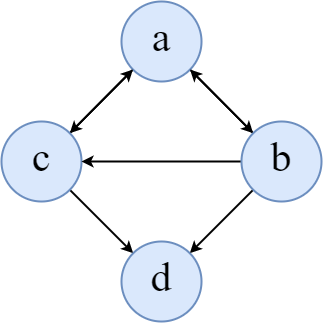
\includegraphics[width=5cm]{images/SYNASC2020_4node_7edge}
		\caption{Egy kommunikációs gráf 4 csúccsal, 3 egyszerű körrel és 1 bonyolulttal}
		\label{abra-synasc2020-4node7edge}
	\end{figure}

	Most az egyszerűség kedvéért elhagyjuk a nem egyszerű kört, és így megkapjuk az egyes ábrán látható  kommunikációs gráf 3 körrel a következő:
	\[ (a,b),(a,b,c),(a,c). \]
	
	Így a gyenge modellje (miután minden egyes klóznak a magába foglalt teljes klózok indexeit kilistázzuk \az{\eqref{eq-teljes-klozok}} képletből):
	\begin{equation*}
		\begin{split}
			WM=\{\{\neg a,b,c\} :6,7,\{\neg b,a,c,d\} :11, \\
			\{\neg c,a,d\} :9,14,\{\neg a,\neg b,c,d\} :3, \\
			\{\neg a,\neg b,\neg c,d\} :1,\{\neg a,\neg b,c,d\} :5\}. \\
		\end{split}
	\end{equation*}

	Például a $ \{\neg a,b,c\} :6,7 $ klózt a 6-os és 7-es klózokból úgy kaptuk, hogy a következőképpen össze éseltük őket:
	$ (\neg a,b,c,\neg d)\wedge(\neg a,b,c,d)\equiv(\neg a,b,c) $
	
	\section{Kiterjesztett erős modell}\label{kif-esm}
	Ezt úgy értem el, hogy ha egy irányított gráf több \textsc{SCC}-ből áll, akkor a neki megfelelő modell mindig kielégíthető, akkor is, ha hozzáadjuk a fekete és a fehér klózokat. Ez a megállapítás független attól, hogy a gráf, melyik modelljét generáljuk le. Akkor is igaz, ha az erős, vagy ha a gyenge, vagy mondjuk a Balatonboglár modell segítségével generáljuk le a neki megfelelő \textsc{SAT} példányt.
	
	Ennek az az oka, hogy az elmélet szerint akkor és csak akkor keletkezik irányított gráfból UNSAT példány, ha az irányított gráf egy \textsc{SCC}-ből áll, azaz erősen összefüggő, és hozzáadjuk a modelljéhez a fekete és a fehér klózokat.
	
	Több esetet is vizsgáltam, amikor azt irányított gráf két \textsc{SCC}-ből áll. Ezeknek az erős modelljét elkészítettem kézzel, illetve programmal is, valamint a WolframAlpha weboldalát használtam fel ezek vizsgálatára.
	
	A WolframAlpha-t már kifejtettem a \ref{kif-wolframalpha-hasznalata}.~fejezetben, így erre itt nem térnék ki minden részlete, a használatával kapcsolatban.
	 
	A legegyszerűbb gráf, aminek erős modelljét vizsgáltam, két \textsc{SCC}-ből áll. Az első \textsc{SCC} az A és a B változókból áll (számokkal kifejezve: 1, 2), a második \textsc{SCC} a C, valamint a D változókból (számokkal kifejezve: 3, 4), oly módon, hogy az első \textsc{SCC}-ből megy él a másodikba. Visszafelé természetesen nem megy él, hiszen akkor az egész gráfunkból egy nagy \textsc{SCC} lenne, amiről tudjuk, hogy egy fekete-fehér \textsc{SAT} probléma. Kutatásom során, azt találtam, hogy függetlenül attól, hogy az A-ból megy él C-be, azaz $ A \rightarrow C $, vagy A-ból megy él D-be: $A \rightarrow D$, vagy B-ből megy él C-be: $B\rightarrow C$, vagy B-ből megy él D-be: $B\rightarrow D$, mind a négy esetben az erős reprezentációnak megfelelő \textsc{DNF} formula a következő volt:
	
	\[ (A\wedge B\wedge C\wedge D)\vee (\neg A\wedge\neg B\wedge C\wedge D)\vee (\neg A\wedge\neg B\wedge\neg C\wedge\neg D) \]
	Azaz: (A és B és C és D), vagy ($ \neg A $ és $ \neg B $ és $ \neg C $ és $ \neg D $) vagy ($ \neg A $ és $ \neg B $ és C és D)
	
	Ezt kaptam mind a négy esetben. Mint látható az első megoldás a fekete klóz negáltja, a második a fehér klóz negáltja, amiket majd kizárunk a végső megoldások közül a fekete és fehér klózok hozzá adásával, ahogy azt előírja az eredeti algoritmus Kusper Gábor és társainak cikkében\cite{am}.
	
	Ugyanakkor a harmadik megoldás nem tűnik el, és ez megfelel az eredeti elméletnek, habár az eredeti elmélet nem magyarázza meg a harmadik megoldás alakját. Ha jól megnézzük, akkor ez a harmadik megoldás: ($ \neg A $ és $ \neg B $ és C és D), azaz az első \textsc{SCC} változói negatívan szerepelnek benne, a második \textsc{SCC} változói pedig pozitívan. Megvizsgáltam több esetet is, az erős modellt legeneráltam programmal, illetve kézzel is, és a fent leírtak mindig tökéletesen beigazolódtak.
	
	Program eredménye:
	
	\begin{tabular}{cccccc}
		p & cnf & 5 & 10 & &   \\
		-1&  2 &  0&   &   &   \\
		-1&  3 &  0&   &   &   \\
		-2&  1 &  0&   &   &   \\
		-3&  4 &  0&   &   &   \\
		-4&  5 &  0&   &   &   \\
		-5&  3 &  0&   &   &   \\
		-1& -2 & -3& -4& -5& 0 \\
		 1&  2 &  3&  4&  5& 0 \\
		-1& -2 & -3& -4& -5& 0 \\
		 1&  2 &  3&  4&  5& 0 \\
	\end{tabular}

	Viszont a program írása közben sokszor futottam bele olyan hibába, hogy egy modell nem úgy néz ki, mint ahogy annak kéne. Ahogyan láthatják a fentebbi táblázaton is, a legenerált \textsc{CNF} fájl a fekete és a fehér klózokat kétszer is tartalmazza. Ezt természetesen kijavítottam és a helyes fájlt írja ki. 
	
	\begin{lstlisting}
def strong_model_literal_gen(G):
	clause = []
	# bw_clause = []
	for i, j in G.edges():
		clause.append(-i)
		clause.append(j)
		clause.append(0.1)
	# for i in G.nodes():
	# 	bw_clause.append(i)
	# for i in bw_clause:
	# 	clause.append(-i)
	# clause.append(0.1)
	# for i in bw_clause:
	# 	clause.append(i)
	# clause.append(0.1)
	return clause
	\end{lstlisting}
	
	Viszont ez csak egy döntés kérdése, mégpedig, hogy milyen klóz halmazt akarok előállítani. A fenti esetben azt láthatjuk, hogy az összegyűjtött klózok halmaza is tartalmazza, és a fájlba író függvény is beleírta. Lehet, hogy az hangzik az elmélethez megfelelő válasznak, hogy a klózok halmaza tartalmazza a fekete-fehér klózokat is, viszont abban az esetben redundanciát is okoz.
	
	
	
	\begin{lstlisting}
def strong_model_literal_gen(G):
	clause = []
	for i, j in G.edges():
		clause.append(-i)
		clause.append(j)
		clause.append(0.1)
	return clause	
	\end{lstlisting}
\begin{equation*}\label{v}
	\vdots
\end{equation*}
\emph{Később, egy másik függvényben, a fájlba íráskor a fekete és a fehér klózok:}
	\begin{lstlisting}
	for n in range(1, N+1):
		file_wm.write('%s ' % -n)
	file_wm.write('%s\n' % 0)
	for n in range(1, N+1):
		file_wm.write('%s ' % n)
	file_wm.write('%s\n' % 0)
	file_wm.close()
	\end{lstlisting}	
	
	Programmal \textsc{CNF} fájlba írt jó eredmény:

	\begin{tabular}{cccccc}
		p & cnf & 5 & 10 & &   \\
		-1&  2 &  0&   &   &   \\
		-1&  3 &  0&   &   &   \\
		-2&  1 &  0&   &   &   \\
		-3&  4 &  0&   &   &   \\
		-4&  5 &  0&   &   &   \\
		-5&  3 &  0&   &   &   \\
		-1& -2 & -3& -4& -5& 0 \\
		1&  2 &  3&  4&  5& 0 \\
	\end{tabular}

	A következő pedig egy WolframAlpha-val készült példa, amibe a ezek a bemeneti adatok:
	\[ ((A\implies B)\wedge(B\implies A)\wedge(C\implies D)\wedge(D\implies E)\wedge(E\implies C)\wedge(A\implies C)) \]
	\textsc{DNF}:
	\[ (A\wedge B\wedge C\wedge D\wedge E)\vee (\neg A\wedge\neg B\wedge C\wedge D\wedge E)\vee (\neg A\wedge\neg B\wedge\neg C\wedge\neg D\wedge\neg E) \]
	
	Mivel a megfigyelésem többször is visszaigazolódott, ezért a következő sejtést fogalmaztam meg:
	
% todo csomópont/node elmagyarázása, definíciója.
	Ha minden irányított gráf, nevezetesen G, két \textsc{SCC}-ből áll, $ S_1 $-ből, és $ S_2 $-ből, akkor ha $ S_1 $-ből legalább egy él vezet $ S_2 $-be, akkor függetlenül az élek számától, illetve, hogy konkrétan az élek melyik $ S_1 $-ben lévő csomópontból, melyik $ S_2 $-ben lévő csomópontba vezetnek, akkor G-nek a \textsc{SAT} modelljének pontosan ez az egy megoldása lesz, amennyiben a modellhez hozzáadjuk a fekete és a fehér klózokat is: $ \neg S_1\wedge S_2 $, ahol $ \neg S_1 $ ez a formula: $\neg A_1 \wedge \neg A_2\wedge\dots\wedge\neg A_k$, ahol $ S_1 $ csomópontjai: $ A_1,A_2,\dots,A_k $, és $ S_2 $ ez a formula: $ B_1\wedge B_2\wedge\dots\wedge B_m $, ahol $ S_2 $ csomópontjai: $ B_1,B_2,\dots,B_m $.
	
	Sajnos a sejtésemet egyelőre nem sikerült bizonyítani, de az általam kipróbált minden példára működött, akkor is, ha az az erős modellt generáltam, akkor is ha a gyengét, akkor is, ha bármely másikat, azaz szerintem ez egy fontos sejtés.
	
		\subsection{Első példa}
	A fenti megfigyelésből az az ötletem támadt, hogy az összes \textsc{SCC}-t egy-egy csomóponttal helyettesítem, azért hogy kisebb bonyolultságú gráfokat kelljen kezelnem, amelyre az általam megírt kódok is gyorsabban futnak.

	Az első út, amit kipróbáltam, az az, hogy hogyan lehet kiegészíteni a legenerált \textsc{SAT} modelleket, oly módon, hogy a fenti ismertetett tulajdonság megmaradjon, azaz $\neg S_1$ és $ S_2 $ megoldás maradjon, de minden egyes \textsc{SCC}-t egy darab változó képviseljen. Ez egy DIMACS fájlban, azt jelenti, hogy nem az \textsc{SCC}-ben szereplő minden csomópontot írom bele számok ként, hanem csak egy számmal jelölöm el azt. Az eredetiből:
	%todo képek milyen szélesek legyenek?
	\begin{figure}[h]
		\centering
		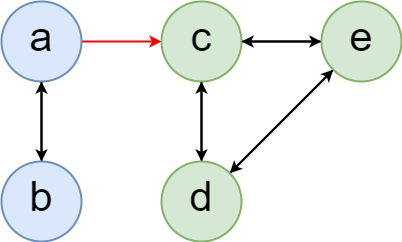
\includegraphics[width=5cm]{images/sajat_pelda_5node_9edge}
		\caption{Eredeti gráf benne az összes \textsc{SCC}.}
		\label{abra-sajatpelda-eredeti-5-9graf}
	\end{figure}
		
	Hosszas próbálkozás után, a következő ötletem támadt:
	
	\begin{figure}[h]
		\centering
		
\includegraphics[width=5cm]{images/sajat_pelda}
		\caption{$ a\leftrightarrow b\equiv x$, azaz egy \textsc{SCC}-t helyettesíthetek egyetlen változóval.}
		\label{abra-sajatpelda-ab-x}
	\end{figure}
	
	% Arra, hogy ezt a modellt leírhatjuk SCC-nként egy node-al, arra én világítottam rá, a konzulensemnek pedig rögtön ez az ötlete támadt.
	% Ha WolframAlpa-ba a következő bemeneti adatokat adjuk meg:
	
	WolframAlpha-ba a bemeneti adatok:
	\[ (A\implies B)\wedge(B\implies A)\wedge(A\vee B \implies X)\wedge(\neg A\vee\neg B\implies\neg X) \]

	% akkor annak a \textsc{DNF}-ben a leegyszerűsített változata:
	\textsc{DNF}-ben a leegyszerűsített változat:
	\[ (A\wedge B\wedge X)\vee(\neg A\wedge\neg B\wedge\neg X) \]	
	Azaz: ((A=>B) és (B=>A) és (A vagy B => X) és ($ \neg A $ vagy $ \neg B $ => $ \neg X $)), ahol az A, és B változókból áll az \textsc{SCC}, valamint X változóval lehet helyettesíteni az \textsc{SCC}-t.
	
	A fenti kiegészítést. úgy lehet megkapni, hogy az \textsc{SCC} fehér klóza implikálja az $ X $ literált, a fekete klóza pedig a $ \neg X $ literált. Ezzel a kiegészítéssel az \textsc{SCC}-nek ugyanúgy csak két megoldása van, mint a kiegészítés előtt. A két megoldás, a fekete, és a fehér hozzárendelése, annyi kiegészítéssel, hogy most már szerepel bennük az X ítéletváltozó is. Azaz a két megoldás: $ (A \wedge B \wedge X) $, valamint $ (\neg A \wedge \neg B \wedge \neg X) $
	
	Ezzel a kiegészítéssel azt lehet nyerni. hogy ha van két \textsc{SCC}, mondjuk $ S_1 $ és $ S_2 $, ekkor $ S_1 $-et az $ X $-el egészítem ki és $ S_2 $-t az $ Y $-al, akkor minden élt, ami $ S_1 $-ből $ S_2 $-be megy, azt le tudom írni egy darab klózzal: $ (X\implies Y) $, azaz $ (\neg X\vee Y) $, ami kisebb \textsc{SAT} modellhez vezethet.
	
	\begin{figure}[h]
		\centering
		
\includegraphics[width=3cm]{images/sajat_pelda_5_9_to_esm}
		\caption{Leegyszerűsített gráf, behelyettesítés után. Kibővített erős modell (\textsc{ESM})}
		\label{abra-sajatpelda-59to-esm}
	\end{figure}

	Ráadásul a modellek általam vizsgált összes tulajdonsága megmarad.
	
	Egy ettől is egyszerűbb megoldás, ha az első \textsc{SCC}-t az 1-es számmal, azaz az $ A $ változóval, a másodikat pedig a 2-es számmal, azaz a B változóval helyettesítem. Azaz rendre egy-egy változót (de mindegyikhez különbözőt) rendelek az erős komponensekhez. Ebből generálok egy erős modellt, majd ennek az erős modellnek a megoldásaimban visszahelyettesítem az \textsc{SCC}-k eredeti változóit a megoldásban kapott előjellel. Így akár nagyon nagy, több ezres irányított gráfok megoldása is milliszekundumok alatt lehetséges.
	
	\begin{figure}[h]
		\centering
		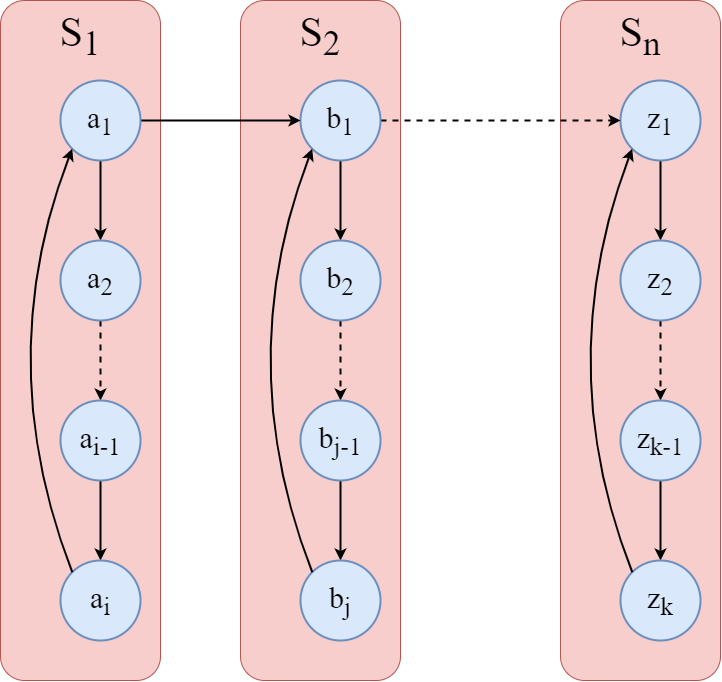
\includegraphics[width=8cm]{images/sajat_pelda-altalanos}
		\caption{Egy gráf leírása, akár mennyi \textsc{SCC} esetén.}
		\label{abra-sajatpelda-altalanos}
	\end{figure}
	
	Ehhez természetesen meg kell találni az összes \textsc{SCC}-t és a köztük lévő kapcsolatokat, ami nem egyszerű feladat. Változatos a gráfok minden formája. Egy általánosított modellt próbáltam meghatározni \ref{abra-sajatpelda-altalanos}.~ábrán, ami az összes lehetséges alakot lefedi.
	
	\begin{figure}[h]
		\centering
		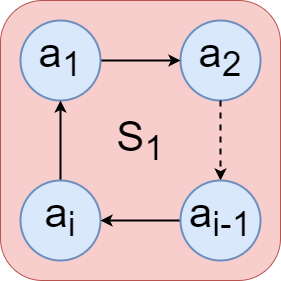
\includegraphics[width=3cm]{images/sajat_pelda-altalanos_scck_a}
		\caption{Egy lehetséges erős komponens alakja (a) változóval jelölve, az $ S_1 $-es erős komponensben.}
		\label{abra-sajatpelda-altalanos_scck_a-verzio}
	\end{figure}
	
	\begin{figure}[h]
		\centering
		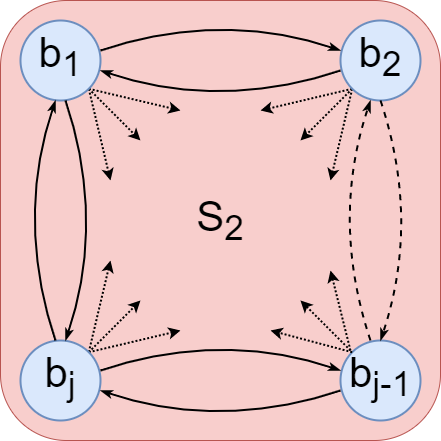
\includegraphics[width=5cm]{images/sajat_pelda-altalanos_scck_b}
		\caption{Egy lehetséges erős komponens alakja (b) változóval jelölve, az $ S_2 $-es erős komponensben.}
		\label{abra-sajatpelda-altalanos_scck_b-verzio}
	\end{figure}
	
%	A képekhez az ihletet \cite{johnson} ábráiból kaptam, amit Tarján algoritmusára írt fel... És a konzulensem ezt kérte volna, hogy implementáljam. Valamint innen tudjuk, hány elemi kör van egy teljes gráfban, mert írt rá egy képletet.
% Beleírhatnám valahova: A kódok előtt összefoglaló, utána kód, és végül a részletezés. Ez a sorrend a kódok leírására.
	
	Az \textsc{SCC}-k megtalálására több módszer is van. Illetve más úton indultam el egy kicsit, mint amit a konzulensem kért tőlem. Szerintem ez nem probléma, hiszen új rávilágítást, és más szemléletet vittem az ő munkájukban tovább. Ezekről kóddal együtt a következő fejezetben részletesebben fejtem ki mondani valóm.
	
\chapter{Szoftver}
	\section{Amiből kiindultam}
	Ebben a fejezetben kiemelt sorok szerepelnek, úgyhogy nem minden részlet van leírva.
	
	A munka, amihez én is hozzá teszem a részemet, egy saját készítésű \textsc{SAT} megoldó a CSFLOCK. Ez ugyan egy Java-ban írt program, viszont én is hozzá tudok tenni, mivel a bemeneti formátum, amivel dolgozik, az egy .CNF fájl. Így tudok ilyen fájlokat generálni a graph\_cnf\_GEN nevű programok segítségével. Ezek különböző verziókban készültek el, ahogyan előre haladtunk. Az alapokat Bíró Csaba egyetemi docens készítette el korábban konzulensemmel közös munkájuk során.
	
	Ez a graph\_cnf\_GEN\_0.8.py \cite{github-py08} fájl névre hallgat. Ebből az alapból kiindulva tanulmányoztam a szerkezetét. Tartalmilag néhány része nem volt tisztán érthető, de már sok minden tisztább és használhatóbb lett az egyel nagyobb verzióban. Nem az összes funkcióját helyettesíti még, hiszen a hangsúlyt a kutató munkára helyeztem, a következő szakaszban foglaltak befejezéséhez.
	
	Még nem sikerült lefordítsam a program egy részét, úgy hogy teljes egészében működjön. Ezt korábban döntöttem el, hogy kihagyom, esetleg csak elhalasztom, hiszen fontos lenne a kód teljes körű működése. Ám ez bonyolultabb feladat, mint gondoltam, hiszen értelmezni kell a modellek pontos működését, és azoknak megfelelőre beállítani, finomhangolni a kódot. 
	
	Mivel \az{\cite{github-py08}} egy korábbi, 2.0 Python-ban készülhetett, ezért egy pár dolog természetesen hibára futott az újabb Python 3.0 feletti verzióban. 
	
	\begin{lstlisting}
for i in xrange(len(clauseSet)):
	if i <> 0:
	\end{lstlisting}

	Néhány kódrészlet pedig azért futott hibára, mert ahogyan az elején megkaptam még nem volt, vagy rosszul volt definiálva néhány változó:
	
	\begin{lstlisting}
isStrConn
graph_dens
g = networkx.DiGraph()
cic = find_cycle(g)
for i in range(0,len(cic)):
	a_cycle.append(cic[i][0])
	\end{lstlisting}

	Az utolsó sor a legérdekesebb, mivel . Sajnos csak jóval később volt halvány sejtésem, hogy ez mit is jelenthet. De a pontos jelentését, és feladatát a rá szánt időben nem tudtam megfejteni. A programban, ugyan ebben a mélységű behúzásban, de kicsit később ezeket a sorokat láthatjuk:
	
	\begin{lstlisting}
if find_cycle(g):
	isCici=len(find_cycle(g))
	\end{lstlisting}

	Ezek alapján már teljesen elvesztem. Az előző, és a felette lévő kódrészletekben háromféle értéket kell vissza adnia a find\_cycle() függvénynek, amire először úgy gondoltam, lehetetlen feladat. A cic változónak értékül adni magát a megtalált köröket. Egy igazságváltozó értéket, gondolom a logika alapján talált-e kört. Majd a harmadik esetben annak a körnek a hosszát vissza adni, vagy hogy mennyi kör van a g irányított gráfban. Mivel ezeket nem tudtam még a kezdetben megválaszolni, emiatt úgy döntöttem, hogy külön fájlban, új verzió számmal elkezdem a nulláról felépíteni a projektet. Sajnos nem jutottam el a teljes kód átdolgozásáig, viszont a következő részben arról írok, ami a dolgát csinálja, érthetően és hiba nélkül.
	
	\section{Kiterjesztett erős modell Python megoldásai}
	
	Nagyon sok verzión ment át a kód, mielőtt idáig eljutott, de végül úgy működik, ahogyan azt elgondoltam és most láthatjuk. Ezért kapott új verzió számot is az átdolgozott rész. Használtam előre megírt könyvtárakat is, amik nagyban segítették a munkámat.

	\begin{lstlisting}
from itertools import tee, islice, chain
import networkx as nx
import pylab
	\end{lstlisting}

	Sorban, ahogyan felhasználtam őket: indexeléshez és pontosabb lista bejáráshoz használom az első sor könyvtárait. A második a legfontosabb munkám során, hiszen minden ami a gráfokhoz kapcsolódik, azt ebből a könyvtárból merítettem. Munkám során a fejlesztők felé is jeleztem saját github repository-juk segítségével néhány példa hiányosságát \cite{link-github-issue}, ami nagyban megkönnyítheti a kód pontos használatának a megértését. Ez a könyvtár segít gráfot építeni, módosítani, keresni benne, rendezni csomópontokat és még sok más hasznos osztályt és függvényt tartalmaz, de ezekről majd később részletesen is beszélek. Valamint még ne feledkezzünk meg az utolsó sorról, ami a gráfok fájlba írását segíti. Rengeteg matematikai műveletet tartalmaz és segít kezelni, formázni a gráfunkat, hogy képeket, és .cnf fájlokat készíthessünk belőle.
	
	A következő részletben a fő elemet láthatjuk. Ebben indítom, el az összes folyamatot és módosítom a bemeneti gráfot.
	
	\begin{lstlisting}
def main():
	edges = []
	
	edges.append((2,1))
	edges.append((1,3))
	edges.append((1,4))
	edges.append((3,2))
	edges.append((4,5))
	edges.append((5,4))
	
	g = nx.DiGraph(edges)
	Literals = expanded_strong_model_literal_gen(g)
	model_to_cnf_file(g, Literals, "ESM")
	Literals = strong_model_literal_gen(g)
	model_to_cnf_file(g, Literals, "SM")
	
main()
	\end{lstlisting}

	Kell egy üres lista, amihez különleges módon adok hozzá. Az éleknek megfelelő számokat a \texttt{NetworkX} fejlesztői egy konvenció alapján adják át az éleket \cite{link-github-issue}, legalább is ebből a beszélgetésből ezt sejtem, és a következő használatot javasolták:
	
	\begin{lstlisting}
edges = []
edges.append(((2,1),(1,3),(1,4),(3,2),(4,5),(5,4)))
	\end{lstlisting}
	
	Én azért használom a hosszabban leírva, mert számomra sokkal átláthatóbb, jobban szerkeszthető és követhető, hogy miből áll a gráfunk. Egy szám egy csomópontnak felel meg. Egy szám páros pedig azt mutatja, hogy a két csomópont közt él van. Ezek listáját átadom a \texttt{NetworkX} irányított gráf generáló algoritmusnak, az elkészült gráfot pedig eltárolom egy változóban. Ezek után saját függvényeimet hívom meg, és elkészítem a modellnek megfelelő literálok halmazát. Végül az elkészült literálokat adom át a Bíró Csaba tanár úr által korábban elkészített cnf fájlt generáló függvénynek.
	
	Amit elkészítettem függvény, az a következőképpen néz ki:
	
	\begin{lstlisting}
def expanded_strong_model_literal_gen(G):
	dagg = nx.condensation(G)
	mem = nx.get_node_attributes(dagg, "members")
	print("members: ",mem)
	clause = []
	edges = list(dagg.edges())
	if len(edges) == 0:
		for i in mem.values():
			while i:
				clause.append(-i.pop())
		clause.append(0.1)
		print("Careful! All are negative literals.")
		return(clause)
	else:
	\end{lstlisting}

	A \texttt{print}-et használom állandó visszajelzésnek, mivel sokszor modell generálást váltok, ezért jó látni, melyikkel dolgozok jelenleg, és milyen rész információkból. A megfelelő bemenetet használtam, azaz csak az éleket kell átadni, és nem mutathat egy csomópont magára. Ezek után a \texttt{NetworkX} könyvtárában a \texttt{condensation} függvényt használva vissza kapom a gráfom kondenzációját. Egy szótárban tárolja az erős komponensekhez hozzárendelt új csomópontokat, és ezeknek az eredeti csomópontjait. A erősen összetett komponenseket Tarján Róbert algoritmusával \cite{tarjan} és Nuutila módosításával \cite{nuutila} találja meg. Ezekkel az adatokkal már egyszerűbb dolgunk van. Ha az egész szótárt bejárjuk, akkor láthatjuk, hogy hány új él van. Ha nincs benne, akkor az egész gráf erős komponens volt, és minden csomópontot negatívként adunk hozzá a klóz halmazhoz.
	
	Ennek else ágában:

	\begin{lstlisting}
for prev, curr in previous(mem.items()):
	if len(curr[1]) > 1:
		for pre, cu in previous(curr[1]):
			if pre == None:
				firs = cu
				continue
			if (pre, cu) in G.edges():
				clause.append(-pre)
				clause.append(cu)
				clause.append(0.1)
			if (cu, pre) in G.edges():
				clause.append(-cu)
				clause.append(pre)
				clause.append(0.1)
			if (cu, firs) in G.edges() and pre != firs:
				clause.append(-cu)
				clause.append(firs)
				clause.append(0.1)
			if (firs, cu) in G.edges() and pre != firs:
				clause.append(-firs)
				clause.append(cu)
				clause.append(0.1)
	if prev == None:
		continue
	if (prev[0], curr[0]) in edges:
		print("edge goes from previous to current")
		for i in prev[1]:
			clause.append(-i)
		for i in curr[1]:
			clause.append(i)
		clause.append(0.1)
	
	if (curr[0], prev[0]) in edges:
		print("edge goes from current to previous")
		for i in curr[1]:
			clause.append(-i)
		for i in prev[1]:
			clause.append(i)
		clause.append(0.1)
	\end{lstlisting}	
	
	Az általam írt függvény fő része végig megy az előző és a jelenlegi elemein a szótárnak. Az első elem előtt nincs semmi, ezért a \texttt{prev} értéke kezdetben \texttt{None}. Viszont ebben az iterációban még a legelső erős komponens elemein végigmegyünk, ha egynél több van és hozzá adjuk annak literáljait a klóz halmazunkhoz. Csak ezek után lépünk a következő iterációra, ahol ugyan ezeket a lépéseket megismételjük, annyi különbséggel, hogy most már az erős komponensek közti éleket is beleírjuk a klóz halmazba. Annyi, hogy a klóz halmazunk tulajdonképpen egy lista, amiben a halmaz elemeit egy különleges értékkel határoltam el.
	
	Ezek után a fájlba a határoló karakter segítésével, egy másik metódussal, a megfelelő \textsc{DIMACS} formátumban írom ki.
	
	\section{Célok a jövőben, további lehetőségek}
	
	Még rengeteg metódus és függvény van, amit meg lehet írni a \cite{github-py08} alapján. Még én magam is terveztem folytatni a modellek átírását az új Python verzióra, valamint azok értelmezését. A jelenlegi kódot is karban lehetne tartani, kitakarítani, szépíteni rajta. Sok lehetőség áll még benne. Remélem a kezem közül olyan kódot adtam ki, amihez nem kell külön a segítségemet kérni. Értelmezhető, és javítható ott, ahol szükséges, hiszen minden kódon lehet szépíteni.

	Ennek hiányosságai még, hogy legyen külön fájlba írva az összes teszt eset. Legyen belőlük több, és legyenek sokoldalúbbak. A teszteseteket lehetne a \texttt{NetworkX} csapatának annotálásával, stílusával és konvenciójával írni a továbbiakban.
	
	A Balatonboglár, Egyszerűsített Balatonboglár és a Gyenge modelleket ki lehet egészíteni, át lehet dolgozni. Ezekhez még nem nyúltam, de szívesen folytatom a munkát későbbiekben, ha még szükséges. Ezek kódba írását, újra fogalmazását lehet folytatni a többi modell mellett.

	Lehet hogy ahogyan én találtam egy félreértés során egy új modellt, úgy más is tovább fejlesztheti az eddigieket, vagy esetleg új ötlettel áll elő.

	A \textsc{SAT} megoldóhoz, amit a konzulensem Java programozási környezetben írt meg és \textsc{CSFLOC} névre hallgat, ahhoz még nem nyúltam hozzá. Úgy tudom abban is lehet fejlesztéseket eszközölni, lásd gyorsabb körkereső algoritmus implementálása \cite[Johnson]{johnson} algoritmusa alapján. A gyenge modellhez pedig minden lehetőség adott, és már csak egy karnyújtásnyira van, hogy annak is láthassuk a végeredményét. Ezek fontos feladatok lennének, hiszen a \textsc{CSFLOCK}-nak teszteléshez szükséges modellekről beszélünk. Ezek az alap pillérei, és mindanyian számítunk arra, hogy ez a projekt tovább haladjon.
	
\chapter*{Összegzés}\addcontentsline{toc}{chapter}{Összegzés}
	Szakirodalomat fordítottam, értelmeztem és dolgoztam fel. Ezekből kiindulva, néhány alap fogalmat leírtam és elmagyaráztam.

	Egy régebbi elmaradt kódot élesztettem, értelmeztem újra. Sok munka árán eljutottam egy modell generálásáig, amire azt hittem a gyenge modell, ám kiderült, hogy az erős modellt általánosítottam. Ehhez a szabályokat, összetételét és a formális megfogalmazását is megcsináltam. Jó fájlokat generál, több tesztesetem is van. Képekkel, ábrákkal próbáltam értehtőbbé, színesebbé tenni a szakirodalmat. Ezekkel elmagyarázni a modellt, és annak működését. Ezek után még külön részleteztem néhány sorát az általam írt kódoknak, hátha így még jobb érthető lesz, és a kód dokumentációjának is megfelel.

	Mivel külső forrásból vannak a linkek, nem én tartom fent az url-ek mögötti weboldalakat, így a linkek idővel elavulhatnak.
	
\chapter*{Köszönet nyílvánítás}

	Nagyon hálás köszönettel tartozom konzulensemnek Dr.~Kusper Gábornak, és tanáromnak Biró Csabának, amiért minden lehetséges módon többször is segítették egyetemi munkámat, megadták az alapokat a szakdolgozatom megírásához, és támogattak, amikor szükségem volt rá. Ezen kívül minden egyetemi tanáromnak köszönöm az építő kritikát, a türelmet és az odaadást, amivel tanítottak, ha ők nincsenek, akkor nem jutottam volna el idáig. Köszönöm a szüleimnek is, hogy megadtak minden anyagi támogatást, hogy ők is türelemmel várták azt, hogy eljussak idáig, és hogy együtt éreztek velem mindvégig. Valamint, hogy ők olvashassák át először szakdolgozatom teljes egészét, ezúton is köszönet a részletes ellenőrzésükért.

	Köszönet a barátnőmnek, és családjának, a barátaimnak a lelki támogatást, és a rengeteg türelmet, amit jópárszor a végletekig húztam, mivel ők hallgatták végig, ahányszor elakadtam valahol, és kérhettem tőlük is segítséget, akár mikor. 
	
	Mindenkinek hogy mindig támogattak, és mögém álltak, ha kellett kemény, de odakellő szavakkal, hogy össze szedjem magam.

\begin{thebibliography}{2}
	\addcontentsline{toc}{chapter}{\bibname}
	%cím, író\\cikk, oldalszám, év
	\bibitem{tarjan}\textsc{Depth-First Search and Linear Graph Algorithms
	\\Robert Tarjan}
	\\SIAM Journal on Computing 1972 1:2, 146-160
	\\\url{https://epubs.siam.org/doi/10.1137/0201010}

	\bibitem{johnson}\textsc{Finding All the Elementary Circuits of a Directed Graph
	\\Donald B.~Johnson}
	\\SIAM Journal on Computing 1975 4:1, 77-84
	\\\url{https://epubs.siam.org/doi/10.1137/0204007}
	
	\bibitem{nuutila}\textsc{Finding the strongly connected components in a directed graph.}
	\\\textsc{E. Nuutila and E. Soisalon-Soinen }
	\\Information Processing Letters 49(1): 9-14, (1994)
	
	\bibitem{am}\textsc{G.~Kusper, T.~Balla, C.~Biró, T.~Tajti, Z.~G.~Yang and I.~Baják, "Generating Minimal Unsatisfiable SAT Instances from Strong Digraphs,"}
	\\2020 22nd International Symposium on Symbolic and Numeric Algorithms for Scientific Computing (SYNASC), 2020, pp. 84-92, doi: 10.1109/SYNASC51798.2020.00024.
	
	\bibitem{sat-solving-50}\textsc{G.~Kusper, C.~Biró and G.~B.~Iszály, "SAT solving by CSFLOC, the next generation of full-length clause counting algorithms,"}
	\\2018 IEEE International Conference on Future IoT Technologies (Future IoT), 2018, pp. 1-9, doi: 10.1109/FIOT.2018.8325589.
	
	\bibitem{github}Saját GitHub oldala a szakdolgozatomnak:
	\\\url{https://github.com/Moss4t/Szakdolgozat}
	
	\bibitem{github-py08}A graph\_cnf\_GEN\_0.8.py fájl ezen a linken található:
	\\\url{https://github.com/Moss4t/Szakdolgozat/blob/main/gen%20py/graph_cnf_GEN_0.8.py}
	
	\bibitem{link-drawio}A draw.io weboldalas elérhetősége:
	\\\url{https://www.draw.io}
	
	\bibitem{link-wolframalpha}A WolframAlpha weboldalas elérhetősége:
	\\\url{https://www.wolframalpha.com}
	
	\bibitem{link-github-issue}Az általam elindított issue GitHub-on
	\\\url{https://github.com/networkx/networkx/discussions/5446}, amiből kiindult beszélgetés, és az issue:
	\\\url{https://github.com/networkx/networkx/issues/5449}		
\end{thebibliography}
	
	% Aláírt, szkennelt nyilatkozat beillesztése a szakdolgozat végére
	%
\includepdf[pagecommand={\thispagestyle{empty}}]{nyilatkozat.pdf}
\end{document}